\label{key}

\documentclass[hidelinks,12pt]{article}
\usepackage{times}
\usepackage[T1]{fontenc}
\usepackage{ragged2e}
\usepackage{adjustbox}
\usepackage{setspace}
\usepackage{babel}
\usepackage{microtype}
\usepackage{graphicx}
\usepackage{float}
\usepackage{subcaption}
\usepackage[utf8]{inputenc}
\usepackage{blindtext}
\usepackage{amsmath}
\usepackage{amssymb}
\usepackage[round]{natbib}
\usepackage{hyperref}
\usepackage[left=2.5cm,top=2.5cm,right=2.5cm,bottom=2.5cm]{geometry}
\DeclareRobustCommand{\hlcyan}[1]{{\sethlcolor{cyan}\hl{#1}}}




\linespread{1.5}


\newtheorem{theorem}{Theorem}[section]
\newtheorem{corollary}{Corollary}[theorem]
\newtheorem{lemma}[theorem]{Lemma}
\newtheorem{definition}{Definition}[section]



\title{\textbf{Inflation Targeting Regime in Brazil: A Replicated Study}}
\author{Caio de Andrade Forcione\footnote{
		Master's Student in Federal University of ABC, Alameda da Universidade, s/nº - Bairro Anchieta - São Bernardo do Campo (email: caio.forcione@ufabc.edu.br). }}
\date{}

\begin{document}
	
	\maketitle
	
	\noindent\rule{17cm}{0.4pt}
	
	\begin{abstract}
	This present work aims to replicate and update data from the article \citet{c15}, in order to demonstrate knowledge in Time Series Analysis. Data from the Brazilian interest rate (Selic), FED Funds, percentage change in the exchange rate, \textit{IPCA} and GDP gap were used, 
	with implementation of VAR models and impulse-response functions.
	\end{abstract}
	\textit{Keywords}: inflation target, interest rate, monetary policy, VAR, impulse response \\
	\textit{JEL classification}: E31, E52, E58
	
	\noindent\rule{17cm}{0.4pt}
	

	
	\section{Introduction}



At the end of the 1990s, Brazil was still trying to get rid of the trauma from the last two decades: hyperinflation. Several plans were made in order to control the main macroeconomic indicators. Under the administration of President Fernando Henrique Cardoso, the Central Bank took measures to guarantee the successful execution of the \textit{Plano Real}, implementing measures of monetary responsibility. as said by \citet{g11}:

\begin{quote}
	\textit{[...] O panorama começou a mudar com a nomeação de Armínio Fraga para o posto de presente do Banco Central. Visto como um profundo conhecedor do mercado financeiro internacional - onde trabalhara durante anos em Nova York - ele escolheu sua equipe e anuncionou duas providências: a elevação da taxa de juros básica; e o início de estudos para a adoção do sistema de metas de inflação, que há anos vinha sendo adotado em diversos países.}\\
	\citet{g11}, p. 176.
\end{quote}

These two measures dictated Brazilian monetary policy for many years, and are still a criterion for evaluating good management by decision-makers. And it will be this period in which I will analyze.\\

This article was elaborate by the foillowing structure: this first section was to elucidate the conjecture and situate the current situation of Brazilian economy. The second section will show the literature about inflation target in Brazil,not only using articles that influence the methodology, but those that debate the same subject. The third section was the intention to show the data used in this article and how it was modify by following the reference article from \citet{c15}. The fourth section explain the methodology of the research, using the VAR model and impulse response function to analyze the shocks that each variable can make on each other. The fifth section show the results from the impulse response study, as well as comparing with the reference article results. The six and final section concludes the article by exposing the main contributions of this research.


	
	\section{Literature Review}
	
The VAR methodology, developed by \citet{s80} 
has a great influence on several macroeconomic researches in the academic area. And this would not be different from the Brazilian case. As was briefly described in the introduction, Brazil before the 1990s was experiencing major instabilities, with economists in their day having trouble figuring out the cause of the country's problems. From the implementation of the \textit{Plano Real} and the inflation targets, it became easier to implement research models used for studies of more developed countries.\\
One of the great researchers of monetary economics in Brazil, Helder Ferreira de Mendonça, there are interesting articles on the topic. in your article \citet{h05}it analyzes the credibility of the Central Bank, also using the VAR methodology. To do so, it uses an article of its own authorship (\citet{h19}) in which he discusses how to measure the credibility of the Central Bank, and thus be able to understand the correlation between the macroeconomic variables. \\
\citet{p11} makes a theoretical and historical study about Brazil from the implementation of inflation targets, showing that it is possible to create comparisons of economic conjunctures with other Latin American countries. In a similar way, the article of the from \citet{nb08} in which it demonstrates the behavior of the exchange rate, interest and Brazilian GDP in the period subsequent to 1999.
	
	
	\section{Data}

The data used in this article is represented by this vector:

\begin{displaymath}
	\mathbb{X}_t' = [\pi_t, e_t, i_t, y_t ]
\end{displaymath}

Being $\pi_t$ the inflation variation from IPCA in porcentage, $e_t$ the variation  from exchange rate from $t$ to $t-1$ and $i_t$ is de difference from Selic rate to the FED Funds ($i_t = r^d - r^f$). $y_t$ is the GDP gap obtained by applying the Hodrick-Prescott Filter\footnote{To apply in R, was used the \textit{mFilter} package and \textit{hpfilter} comand.}. This filter (or decomposition) is a mathematical tool with the intention to smooth the time series data. It is useful to remove cyclic component, and change the interpretation of the data, now seen  as how the GDP deviates from its trend. All variables was selected from January 2000 to February 2020 with monthly observations, in a total of 242 per variable. Some outliers had to be removed, as exchange rate data from July 2002 to Semptember 2002 and IPCA data from November 2002 to January 2003.\\



	\begin{figure}[H]
		\centering
		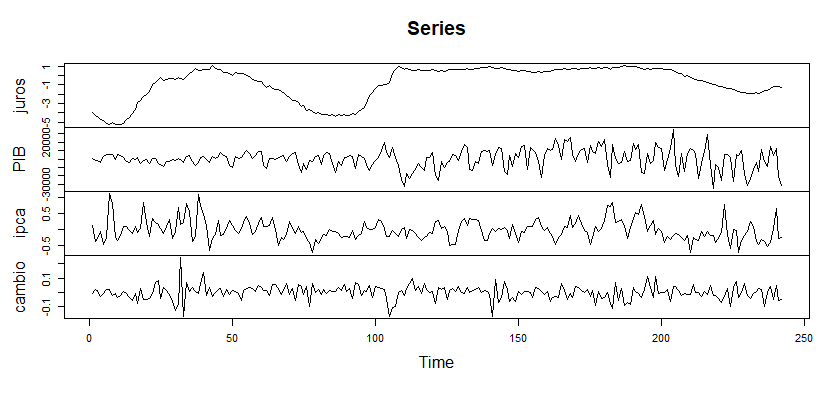
\includegraphics[width=1.0\linewidth]{Rplot}
		\caption{Series before ADF tests and seasonalize.}
		\label{fig:rplot}
	\end{figure}

First, the stationarity of the series was tested, by the ADF criteria. The exchange rate, inflation and GDP showed to be stationary, with $\tau_3 < -3,13$, $\phi_2 > 4,07$ and $\phi_3 > 5,47$. The interest rate $i_t$ proved to be non-stationary, and therefore will be used by it first difference, as the reference article did. And it is important to say that the gap GDP had a seasonal component, so it was included in the model.



\begin{figure}[H]
	\centering
	\includegraphics[width=1.0\linewidth]{"../2. Dados/Rplot01"}
	\caption{Series after ADF tests and seasonalize.}
	\label{fig:rplot01}
\end{figure}



	\section{Metodology}

The methodology of this article is the VAR (Vector Auto Regression) developed by \citet{s80}. The model can be represented as:

\begin{displaymath}
	\mathbb{A} \mathbb{X}_t = \mathbb{B}_0 + \sum_{i = 1}^{p} \mathbb{B}_i \mathbb{X}_{t-i} + \mathbb{B} \epsilon_t
\end{displaymath}

Where $\mathbb{A}$ is a $nxn$ matrix defined by the contemporary restrictions, $\mathbb{B}_0$ is a constant vector, $\mathbb{B}_i$ is a matrix $nxn$ of constants, $\mathbb{B}$ is a diagonal matrix dimension $n$, $\mathbb{X}$ is a matrix $nxn$ of endogenous variables and $\epsilon_t$ is a vector of random schocks, with white noise proprieties. However, as the reference article say, researchers are insterested in the interrelation between variables, using impulse-response functions, represented by:

\begin{displaymath}
	\mathbb{X}_t = \mathbb{C}_0 + \epsilon_t + \sum_{i = 1}^{p} \Psi_i \epsilon_{t-i}
\end{displaymath}

Where $\mathbb{C}$ are the average of the process and $\Psi_i$ is the impact multiplier of a change in $\epsilon$ on the endogenous variables.\\

Now, to especify the model I needed to define how many lags it should have. From each serie, it was lagged 13 periods. To  selection of the VAR especification, I looked at different criteria, as Akaike Information Criterion (AIC), the Hannan-Quinn Criterion (HQ), the Schwarz Criterion (SC) and the Akaike's Final Prediction Error Criterion (FPE).

\begin{table}[H]
	\centering
	\begin{tabular}{|c|c|c|c|}
		\hline
		AIC(n) & HQ(n) & SC(n) & FPE(n) \\ \hline
		4      & 2     & 1     & 4      \\ \hline
	\end{tabular}
\end{table}


The only way to compare the results from \citet{c15} is to look at the Schwarz Criterion, the one that they used. Equal to \citet{c15} analysis, I had the same result with a one period lag\footnote{It is possible to notice in Figure 3 an autocorrelation with a lag in the eighth period of the interest rate, but it is possible that is a spurious correlation.}.

\begin{figure}[H]
	\centering
	\includegraphics[width=0.7\linewidth]{"../2. Dados/Rplot02"}
	\caption{Autocorrelation function from the model VAR(1).}
	\label{fig:rplot02}
\end{figure}
	
	\section{Results}
	
Before showing the results, it is important to say that the reference article had an insight to order the effect of the macroeconomic variables, as:


\begin{center}

$y \rightarrow \pi \rightarrow i \rightarrow e$

\end{center}

Now is possible to show the results graphics from the impulse-response model:

\begin{figure}[H]
	\centering
	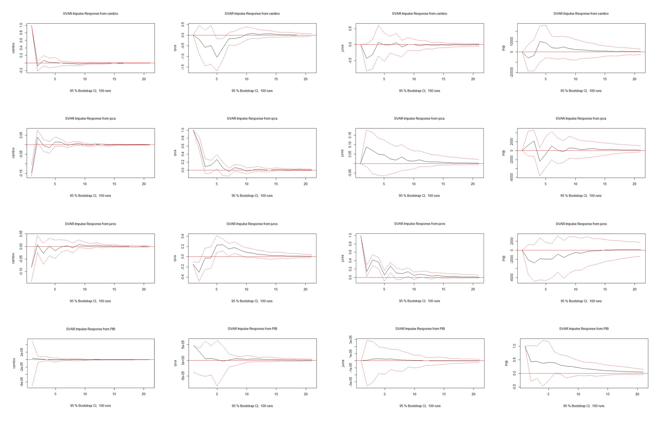
\includegraphics[width=0.7\linewidth]{irf}
	\caption{Impulse-Response Grafics}
	\label{fig:irf}
\end{figure}

Most of the conclusions was correlated with the reference article. Analysing the macroeconomic variables shocks, the exchange rate showed an instant impact on inflation by reducing the prices and oscillating the impact on the gap GDP and differential interest rate. By raising the differential interest rate (increasing SELIC over FED Funds) decreases inflation, but had a different behavior after the first periods. Since we had in Brazil a lower interest rate volatility in comparison to inflation, showed a positive effect before smoothing the impact, that it was not showed in the reference article. The shock from the differential interest rate in the gap GDP cause a negative effect, and been smoothed out after 10 periods. 
	
	\section{Conclusions}

In this article, an update was made to the results founded by \citet{c15}. It was observed that the IPCA, the GDP gap and the exchange rate are stationary series, while the national interest difference with the foreign one was first-order integrated, therefore, using its first difference. I used the VAR model and by Schwarz Criterion, the best model is a one-period lagged.\\

 The results of the impulse-response model were correlated with what was done by the authors, with interest rate having negative impact on inflation, GDP gap and exchange rate, being coherent with the article and the theory.





	\bibliographystyle{apa}
	\bibliography{reference}

\clearpage










	
\end{document}